\documentclass[a4paper,11pt]{article}

\usepackage[left=2cm,text={17cm, 24cm},top=3cm]{geometry}
\usepackage[utf8]{inputenc}
\usepackage{times}
\usepackage[czech]{babel}
\usepackage{graphics}

\begin{document}
\begin{center}
\Huge
\textsc{Vysoké učení technické v~Brně\\
}Fakulta informačních technologií\\
\vspace{\stretch{0.382}}
\LARGE Implementace interpretu imperativního jazyka IFJ16 \\
\Huge Tým 021, varianta a/3/I\\
\vspace{\stretch{0.309}}

\Large Vedoucí:	Kyzlink Jiří 	(xkyzli02)\\
				Kubiš Juraj		(xkubis15)\\
				Korček Juraj	(xkorce01)\\
				Kubica Jan		(xkubic39)\\
				Kovařík Viktor	(xkovar77)\\

\vspace{\stretch{0.309}}

\end{center}
{\Large \today \hfill
Brno}
\thispagestyle{empty}

\newpage

\tableofcontents

\newpage
\section{Úvod}
V této dokumentaci naleznete popis a návrh interpretu jazyka IFJ16, který je velmi zjednodušenou podmnožinou jazyka Java SE 8, což je staticky typovaný objektově orientovaný jazyk. Vybrali jsme si variantu varianta a/3/I, kde jsme měli za úkol přidat do interpretu vestavěnou funkci find, která využívala Knuth-Morris-Prattův algoritmus a funkci sort, kterou jsme měli implementovat tak, aby využívala shell sort.

--bude ještě doplněno-

\section{Syntaktický analyzátor}

\section{Sémantický analyzátor}

\section{Lexikální analyzátor}

\section{Interpret}

\section{Vestavěné funkce}
\subsection {vestavěné funkce v IAL.c}
--nevím jestli rozdělovat na podsekce ještě měnší nebo ne--
\subsubsection {find}

\subsubsection {sort}
\section{Testy}
Testovali jsme buď součásti - \textit{unit testy}, kde jsme zkoušeli, zda daná funkce správně reaguje na vstupy. Unit testy si dělal každý sám a podle potřeby. Bylo zvykem v Makefile pro unit test udělat zvláštní target, kde se kromě samotné kompilace ještě prováděl \textit{valgrind} test pro ověření možných \textit{memory leaků}. 

Dále jsme dělali ještě systémové testy. To byly vlastně testy samotného interpretu a porovnávání jeho výstupu s výstupem Javy SE 8 s přidanou kompatibilitou s jazykem IFJ16. Test byl vytvořen jako samostatný bash script, který se volal z Makefile. Ve složce test/input/ byly růžné programy v jazyce IFJ16 ve formátu \textit{navratovykod\_nazevprogramu.ifj16} s možností přidání ještě souboru se stejným formátem, ale koncovkou .in, kde byla možnost dát vstup na \textit{stdin}. Daný skript pak prošel složku, zjistil, zda jsou v ní obsaženy i soubory typu .in pro právě intepretovaný kód. Pokud byla předpokládaná návratová hodnota 0 (chyby ifj16 interpretu nemělo smysl překládat v javě a porovnávat), došlo k interpretaci kódu v javě i ifj16 interpretu s následným porovnání návratových kódů a výstupů. Vše se zapisovalo do logu, který se nacházel ve stejné složce \textit{input} jako interpretovaný kód. Obrázek níže zobrazuje výsledky testování v průběhu raných fází interpretu.\\

\scalebox{0.77}{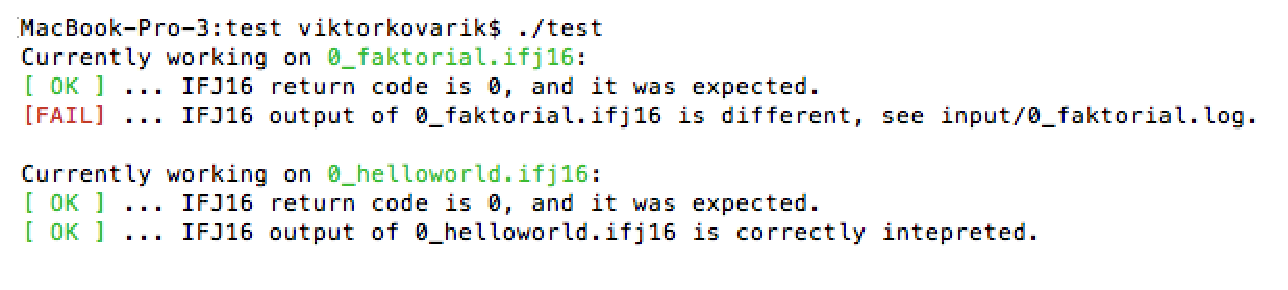
\includegraphics{testy-interpretu.eps}}

\end{document}